\documentclass[a4paper,11pt]{article}
\usepackage[T1]{fontenc}
\usepackage[utf8]{inputenc}
\usepackage{lmodern}
\usepackage{bookmath}
\usepackage{amsmath}
\usepackage{graphicx}
\title{HW 6: Physics 545}
\author{Ben Rosemeyer}

\begin{document}

\maketitle

\section*{1a}
To show this relation we need use the fact that the distribution function $n(\epsilon_p) = n(\epsilon_p-\mu) = n(\xi_p)$ is a function of $\epsilon_p$ and $\mu$ so that $\frac{\delta n_p}{\delta \epsilon_p} =\frac{\delta \xi_p}{\delta \epsilon_p} \frac{\delta \mu}{\delta \xi_p}\frac{\delta n_p}{\delta \mu} = -\frac{\delta n_p}{\delta \mu}$. 

As $q\rightarrow 0$, the differences in the numerator and denominator of the density-density correlation become differentials so:
\bea
\chi(q\rightarrow 0)& =& -\int\limits_{-\infty}^\infty \frac{dp}{2\pi\hbar} \frac{\delta n_p}{\delta \epsilon_p}
=  \int\limits_{-\infty}^\infty \frac{dp}{2\pi\hbar} \frac{\delta n_p}{\delta \mu}
 =  \frac{1}{\delta \mu} \int\limits_{-\infty}^\infty \frac{dp}{2\pi\hbar} \delta n_p \\
 \boxed{\chi(q\rightarrow 0) = \frac{\delta n}{\delta \mu}}
\eea
Where we used the relations above and the definition of $\delta n = \int\limits_{-\infty}^\infty \frac{dp}{2\pi\hbar} \delta n_p$. Thus we have the desired result $\kappa_T = \frac{1}{n^2}\frac{\delta n}{\delta \mu} = \frac{1}{n^2}\chi(q\rightarrow 0)$
\section*{1b}
We can do the integral for $\chi$ noting that the distribution functions limit the integration to two intervals $[-p_f-q/2,-p_f+q/2]$ (+ from $n_{p+q/2}$), $[p_f-q/2,p_f+q/2]$ (- from $n_{p-q/2}$).
\bea
\chi(q)& =& - \int\limits_{-\infty}^\infty \frac{dp}{2\pi\hbar} \frac{n_{p+q/2} - n_{p-q/2}}{\epsilon_{p+q/2} - \epsilon_{p-q/2}} \\
	& = & - \int\limits_{-p_f-q/2}^{-p_f+q/2} \frac{dp}{2\pi\hbar} \frac{1}{2qp} + \int\limits_{p_f-q/2}^{p_f+q/2} \frac{dp}{2\pi\hbar} \frac{1}{2qp} \\
\boxed{\chi(q) =  \frac{1}{2\pi\hbar q}\,ln\bigg|\frac{p_f+q/2}{p_f-q/2} \bigg|}
\eea

The discontinuity is at $q^* = 2p_f$ and we define $\chi_0 = \frac{1}{2\pi\hbar p_f}$

\begin{figure}[t]
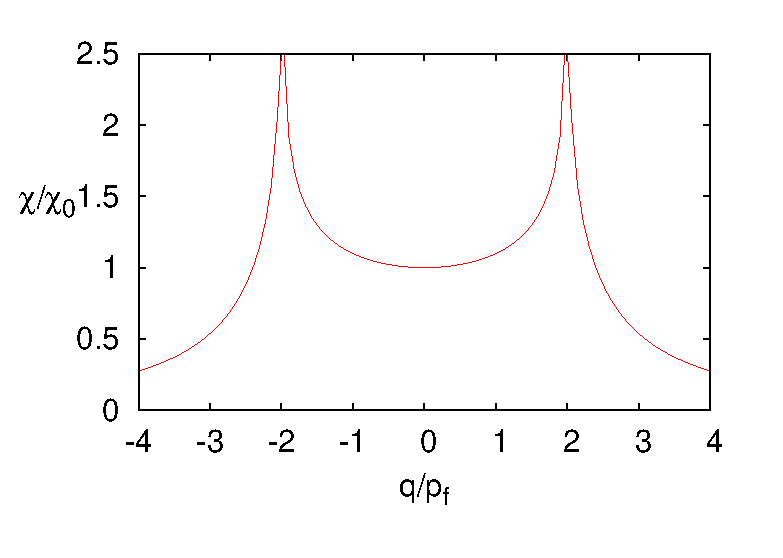
\includegraphics[scale = 0.7]{fig.eps}
\end{figure}
\section*{2}
The Hamiltonian can be written as $\mathcal{H} = \sum\limits_{q>0, \sigma} \epsilon_{q\sigma} \ha^\dagger_{q\sigma} \ha_{q\sigma}$, where $\sigma = \{s,c\}$ denotes the spin or charge channel, and the energies are $\epsilon_{q\sigma} = q v_\sigma$. Here it is important to note that the operators $\ha_{q\sigma}$ are BOSONIC and the distribution function $n_{q\sigma}=<\ha^\dagger_{q\sigma} \ha_{q\sigma}> = \frac{1}{e^{(\epsilon_{q\sigma}-\mu)/T} - 1}$, which requires $\epsilon_{q\sigma}>\mu$ ( $q>\mu/v_\sigma$)

To calculate the specific heat ($C_v = T \frac{\delta S}{\delta T}$) we start by writting the entropy S:
\bea
S = \sum\limits_{q\sigma} (n_{q\sigma} + 1) \, ln(n_{q\sigma} + 1) - n_{q\sigma}\, ln(n_{q\sigma}) \\ 
\delta S = -\sum\limits_{q\sigma}  \delta n_{q\sigma}\, ln\bigg[\frac{n_{q\sigma}}{n_{q\sigma} + 1}\bigg]  \\
\delta S = \sum\limits_{q\sigma}  \delta n_{q\sigma}\, (\epsilon_{q\sigma}-\mu)/T 
\eea
Plugging the equation for $\delta S$ into $C_v$ we see that there will be a term like $\frac{\delta n_{q\sigma}}{\delta T}$. If we neglect higher order corrections to the temperature deviations (ie $\frac{\delta}{\delta T} (\epsilon_{q\sigma} - \mu) \approx 0$) we have:
\be
\frac{\delta n_{q\sigma}}{\delta T} = \frac{e^{(\epsilon_{q\sigma}-\mu)/T}(\epsilon_{q\sigma}-\mu)/T^2}{(e^{(\epsilon_{q\sigma}-\mu)/T} - 1)^2} = \frac{(\epsilon_{q\sigma}-\mu)/T^2}{sinh^2(\epsilon_{q\sigma}-\mu)/2T)}
\ee
The specific heat is
\bea
C_v & = & \sum\limits_{q\sigma} \frac{\big[(\epsilon_{q\sigma}-\mu)/T\big]^2}{sinh^2(\epsilon_{q\sigma}-\mu)/2T)} \\ 
& = & \sum\limits_{\sigma}\int\limits_{\mu/v_\sigma}^\infty\frac{dq}{2\pi\hbar} \frac{\big[(\epsilon_{q\sigma}-\mu)/T\big]^2}{sinh^2(\epsilon_{q\sigma}-\mu)/2T)} \\
& = & 8T\sum\limits_{\sigma}\int\limits_{0}^\infty\frac{dx}{2\pi\hbar v_\sigma} \frac{x^2}{sinh^2(x)} \\
\boxed{C_v = \frac{2T\pi}{3\hbar} \sum\limits_{\sigma}\frac{1}{v_\sigma}}
\eea

We can compare this result to the 1D fermi liquid case by following the notes from class. Doing this we arrive at the following equation for $C_v$ 

\bea
C_v &=& 4 \int\limits_{0}^{\infty} \frac{dp}{2\pi\hbar} [(\epsilon_p-\mu)/T]^2 cosh^{-2}[(\epsilon_p-\mu)/2T] \\
    &=& \frac{\sqrt{m}}{\sqrt{2}\pi\hbar} \int\limits_{0}^{\infty} \frac{d\epsilon}{\sqrt{\epsilon}} [(\epsilon-\mu)/T]^2 cosh^{-2}[(\epsilon-\mu)/2T] \\
    &=& \frac{4T\sqrt{2m}}{\pi\hbar} \int\limits_{-\mu}^{\infty} \frac{dx}{\sqrt{Tx + \mu}} x^2 cosh^{-2}[x] 
\eea
At this point we note that $cosh^{-2}[x]$ is strongly peaked near x=0 allowing us to extend the lower integration limit to $-\infty$. We can also taylor expand for small $Tx$ so that $\frac{1}{\sqrt{Tx + \mu}}\approx \frac{1}{\sqrt{\mu}}$ and set $\mu = \epsilon_f$. Thus, the leading order temperature behavior of $C_v$ for 1D Fermi liquid is:
\be
\boxed{\frac{4T \pi}{3 v_f \hbar}}
\ee
The temperature dependence is the same! In fact the results are identical if the spin/charge velocities satisfy $v_c = v_s = v_f$
\end{document}
